%!TeX encoding = utf8
%!TeX spellcheck = it_IT

\documentclass[a4paper, 12pt]{article}

\usepackage[T1]{fontenc}
\usepackage[utf8]{inputenc}
\usepackage[italian]{babel}

\usepackage{amsmath, amssymb, amsthm}
\usepackage{geometry, emptypage}
\usepackage{graphicx, subfig}
\usepackage{braket}
\usepackage{parskip}

\title{Modulo 6}

\begin{document}
\maketitle
In questo modulo ci concentriamo sullo studio della termodinamica di una teoria
di campo, usando il formalismo del path integral.

\section{Termodinamica del campo scalare libero}
Per prima cosa abbiamo studiamo la termodinamica del campo scalare libero,
descritto dalla lagrangiana

\begin{equation}
\mathcal{L} = \frac{1}{2}\partial_{\mu}\phi \partial^{\mu}\phi - \frac{1}{2}m^2 \phi^2
\label{lagrangiana_campo_scalare}
\end{equation}

L'azione associata all'equazione \ref{lagrangiana_campo_scalare} è
\begin{equation}
S=\int d^4x \mathcal{L}
\end{equation}

Per studiare questa teoria a temperatura finita usiamo la funzione di partizione
\begin{equation}
Z(T) = \int \mathcal{D} \phi_{(s)} \bra{\phi_{(s)}} e^{-\beta \hat{H}}
        \ket{\phi_{(s)}} = \mathcal{N} \int \mathcal{D}\phi \; e^{-S_E[\phi]}
\label{funzione_partizione_campo_scalare}
\end{equation}
dove $\phi_{(s)}$ indica che l'integrazione è sulle configurazioni spaziali
del campo e $S_E$ è l'azione euclidea, che si ottiene con la rotazione di Wick
$t \rightarrow -i\tau$:

\begin{equation}
S_E = \int_0^\beta d\tau \int d^3x (\partial_{\mu}\phi \partial_{\mu}\phi + m^2)
\end{equation}

Il secondo integrale dell'equazione \ref{funzione_partizione_campo_scalare} si
estende a tutte le configurazione di campo nello spazio-tempo euclideo $(\vec{x}, \tau)$,
con $\tau \in [0, \beta]$ e con condizioni periodiche al bordo in direzione temporale
$\phi(\vec{x}, \beta) = \phi(\vec{x}, 0)$.

Ricordando che $\beta = 1 / T$, e il limite per temperatura nulla (teoria nello
stato di vuoto) si ottiene per $\beta \rightarrow \infty$.

\paragraph{Discretizzazione teoria}
Abbiamo lavorato in $1 + 1$ dimensioni: una dimensione temporale e una
spaziale.

Discretizzando la teoria su reticolo con latting-spacing $a$ uniforme sia
nello spazio che nel tempo, abbiamo introdotto le variabili adimensionali
(indicate con "\^{}") $\hat{m} \equiv am, \hat{\phi} \equiv a \phi$,
dove \emph{m} e $\phi$ sono la massa fisica e il campo fisico.
Attuando quindi le sostituzione
\begin{equation}
\int d^4x \rightarrow \sum_n a^4; \qquad
\partial_{\mu}f(n) \rightarrow \frac{f(n+\hat{\mu}) - f(n)}{a}
\end{equation}

dove $n+\hat{\mu}$ è il sito la cui coordinata $\mu$-esima è aumentata di uno
rispetto al sito n, otteniamo:

\begin{align}
S_E^L &= \sum_n \left[ \sum_{\mu} \frac{1}{2} \left(\hat{\phi}(n+\hat{\mu})-
            \hat{\phi}(n) \right)^2 + \frac{1}{2} \hat{m}^2 \hat{\phi}(n)^2 \right] \\
      &= \frac{1}{2} \sum_n \left[ (\hat{m}^2 + 4) \hat{\phi}(n)^2 - 2 \sum_{\mu}
            \hat{\phi}(n)\hat{\phi}(n+\hat{\mu}) \right]
\end{align}

I campi nel nostro modello hanno la seguente distribuzione di probabilità:
\begin{equation}
\mathcal{P}[\hat{\phi}] \prod_n d \hat{\phi}(n) =
e^{-S_E^L[\hat{\phi}]} \prod_n d \hat{\phi}(n)
\end{equation}

% Fra i parametri adimensionali del modello ci sono la dimensione del reticolo e $\hat{m}$
Dato che $\hat{m} = am$, per fare il limite al continuo bisogna mandare
$\hat{m} \rightarrow 0$.
Ricordando inoltre che la temperatura è
\begin{equation}
T= \frac{1}{N_t a} \rightarrow \frac{T}{m} = \frac{1}{N_t \hat{m}}
\end{equation}

per fare il limite al continuo a temperatura fissa:
$N_t \propto 1/\hat{m}$

\paragraph{Energia del campo scalare al variare della temperatura}
Abbiamo posto $\hat{m}=0.05$ e calcolato l'energia del campo
variando la temperatura, cioè per diversi valori di $N_t$.

Per calcolare l'energia del campo abbiamo utilizzato in due modi distinti:
\begin{enumerate}
\item il reticolo anisotropo
\item il metodo dell'anomalia di traccia
\end{enumerate}

Tuttavia come prima cosa abbiamo deciso che tipo di algoritmo utilizzare.
Ponendo quindi $N_t=30$ abbiamo utilizzato un heatbath come algoritmo di simulazione,
seguito da N overrelaxation, facendo ogni volta 120 K spazzate di heatbath
su tutto il reticolo. In tabella \ref{benchmark_campo_scalare} vediamo
il tempo impegato e gli errori dell'energia e dell'anomalia di traccia (a meno
di rinormalizzarle e dividerle per $T^2$),
spiegate nei prossimi paragrafi, in funzione del numero di overrelaxation
utilizzate dopo ciascun heatbath.

\begin{center}
\begin{tabular}{ c | c | c | c }
\label{benchmark_campo_scalare}
$N^{\circ}$ overrelaxation & tempo impiegato (s) &
$\delta \epsilon / N_t ^ 2 \; (10^{-5})$ &
$\delta (\epsilon - p) / N_t ^ 2 \; (10^{-5})$ \\
\hline
0 & 27 & 5.9 & 6.4 \\
1 & 29 & 5.7 & 1.1 \\
2 & 31 & 5.8 & 0.70 \\
3 & 33 & 5.7 & 0.62 \\
4 & 35 & 5.7 & 0.56 \\
5 & 36 & 5.7 & 0.52 \\
6 & 38 & 5.8 & 0.51 \\
7 & 40 & 5.8 & 0.50 \\
8 & 41 & 5.7 & 0.50
\end{tabular}
\end{center}

Per l'energia interna non abbiamo un guadagno sostanziale dopo la prima
overrelaxation, mentre guardando l'anomalia di traccia abbiamo deciso di fare
un heatbath seguito da 5 overrelaxations, in quanto un numero maggiore di
heatbath non avrebbe portato ad un guadagno sostanziale.

\paragraph{Reticolo anisotropo}
Vogliamo calcolare l'energia del campo scalare
\begin{equation}
U=-\left(\frac{\partial \log Z}{\partial \beta} \right)_V
\end{equation}
ma dobbiamo fare attenzione a fare correttamente la derivata a volume spaziale
costante.

Introducendo una diversa dimesione del reticolo temporale e spaziale:
$a_s = a$ e $a_t = \xi a$, abbiamo $\beta = N_t a_t = \xi N_t a$.
La derivata rispetto a $\beta$ con $N_t$ e $a$ costanti diventa:
\begin{equation}
\frac{\partial}{\partial \beta} = \frac{1}{N_t a} \frac{\partial}{\partial \xi}
\end{equation}

ottenendo:
\begin{equation}
U = \frac{1}{N_t a} \left< \sum_n \left(\frac{1}{2}\hat{m}^2 \hat{\phi}^2(n) +
\sum_{\mu=1}^3 \frac{1}{2} \left( \hat{\phi}(n+\hat{\mu})- \hat{\phi}(n) \right) ^2
- \frac{1}{2 \xi^2} \left( \hat{\phi}(n+\hat{0})- \hat{\phi}(n) \right)^2 \right)\right>
\end{equation}

ponendo ora $\xi=1$ e \emph{rinormalizzando} l'energia a basse T, sottraendo
alla quantità mediata intensiva, indipendente da $N_t$, la stessa quantità a
a temperatura più bassa, otteniamo l'energia del campo:

\begin{equation}
E = N_t^2 (\left< O_1+O_2-O_3 \right>_T- \left< O_1+O_2-O_3 \right>_{T=0})/2
\end{equation}

Dove $O_1, O_2, O_3$ sono le variabili riportate nel codice di esempio fornito
durante il corso.
Nella prima parte del nostro esperimento come detto abbiamo utilizzato $m=0.05$,
$N_s=80$ e utilizzato $N_t = 80$ per rinormalizzare, abbiamo preso un numero
diverso di misure per ogni run dell'algoritmo a $N_t$ diverso, poiché per
$N_t$ maggiori avevamo un maggior errore, abbiamo preso più misure per questi
dati, in modo che tutti gli errori fossero confrontabili.

Mostriamo i risultati in figura \ref{campo_scalare_massa_fissa}:
\begin{figure}
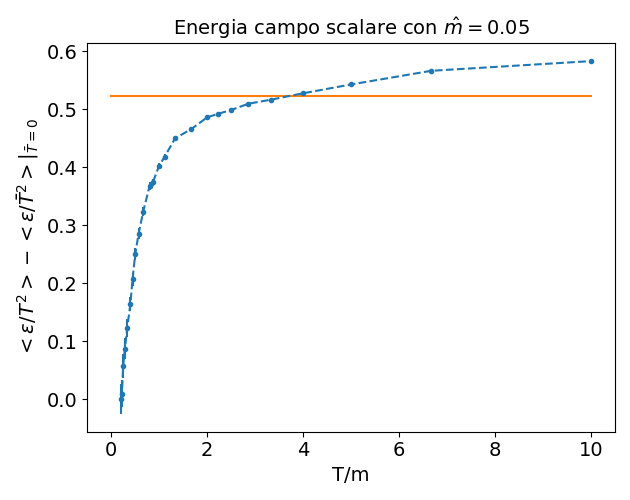
\includegraphics[width = \linewidth]{../figure/massa_fissa.png}
\caption{Energia del campo al variare della temperatura,
calcolata con reticolo anisotropo, in arancione il risultato atteso
per alte temperature (teoria massless).}
\label{campo_scalare_massa_fissa}
\end{figure}

Abbiamo calcolato l'errore prendendo la deviazione standard delle misure
intorno alla media delle stesse, divise per la radice del numero di misure e
poi moltiplicando per $\sqrt{1+2 \tau_{int}}$ per tenere conto
dell'autocorrelazione della mia catena di Markov $O=O_1+O_2-O_3$.

\begin{equation}
\delta \left< \mbox{O} \right> = \mbox{std(O) / len(O)} \times \sqrt{1+2 \tau_{int}}
\end{equation}

Ad alte temperature ci aspettiamo che il sistema si comporti come una teoria di
campo scalare massless, cioè che l'energia tenda a $\pi / 6$.
In realtà vediamo che il nostro risultato sovrastima leggermente le aspettative,
e questo è dovuto, come vedremo nel prossimo paragrafo, al non lavorare
nel limite al continuo.

\paragraph{Limite al continuo per alte temperature}
Per il punto a temperatura più alta in figura \ref{campo_scalare_massa_fissa},
$T/m=10$, (qui $N_t = 2$) abbiamo fatto il limite al continuo:
abbiamo diminuito $\hat{m}$ e aumentato $N_t$, in modo che $\hat{m} \times N_t = 1 / 10$,
in figura \ref{campo_scalare_temperatura_fissa}:
\begin{figure}
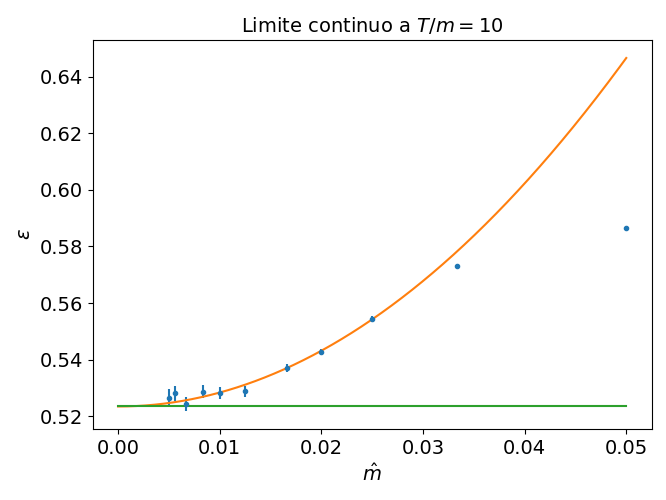
\includegraphics[width=\linewidth]{../figure/massa_variabile.png}
\caption{Energia del campo per $T/m=10$, facendo il limite al continuo.}
\label{campo_scalare_temperatura_fissa}
\end{figure}

Nuovamente abbiamo calcolato gli errori avendo cura di tenere conto
dell'autocorrelazione fra le misure.

L'errore dovuto alla discretizzazione ci aspettiamo vada come $a^2$ quindi
un andamento quadratico in $\hat{m}$, che è quello che osserviamo per $N_t$ grandi.
Faccendo un fit escludendo gli ultimi due punti, che escono dal range di $a$
per cui l'andamento è quadratico, otteniamo una stima dell'energia del campo
pari a $\epsilon = 0.5235(9)$ a $T/m = 10$ contro un risultato teorico atteso
di $\pi / 6 = 0.5236$ per $T/m \rightarrow \infty$.

Il risultato ottenuto nel limite al continuo si abbassa si avvicina alla
previsione teorica, e diventa addirittura una sottostima. Questo perché
stiamo lavorando a temperatura finita di $T/m=10$ e non a temperatura infinita.

\paragraph{Anomalia di traccia}
Un modo più generalizzabile per calcolare l'energia del campo scalare,
utilizzabile anche per teorie più complesse (QCD) è il metodo dell'anomalia
di traccia.

\begin{equation}
- \frac{\partial}{\partial \hat{m}} \log Z
= \frac{1}{m} \left( -\frac{\partial \log Z}{\partial \beta}
    \frac{\partial \beta}{\partial a} -\frac{\partial \log Z}{\partial V}
    \frac{\partial V}{\partial a}\right)
= \frac{1}{m}(N_tU-N_tpV)
= \frac{N_t \times V}{m} (\epsilon - p)
\end{equation}

dove $p$ è la pressione
\begin{equation}
p=-\frac{\partial F}{\partial V} = T \frac{\partial \log Z}{\partial V}
\end{equation}

Dalle quantità termodinamiche possiamo legare la derivata della pressione
e l'anomalia di traccia:
\begin{equation}
T \frac{\partial}{\partial T} \left( \frac{p}{T^2} \right) = \frac{\epsilon - p}{T^2}
\label{anomalia_traccia}
\end{equation}

Abbiamo calcolato $(\epsilon - p) / T^2$ sottraendo l'energia di vuoto (rinormalizzando):
\begin{equation}
\left( \frac{\epsilon - p}{T^2} \right)_R = N_t^2(\left<O_1 \right>_{N_t}
- \left<O_1 \right>_{\bar{N}_t})
\end{equation}

Con $\bar{N}_t \gg N_t$, nella simulazione abbiamo scelto $\bar{N}_t = 50$.

Ottenuto $\epsilon - p$ (ricordo che sono in 1+1 dimensioni),
posso integrare direttamente l'equazione \ref{anomalia_traccia} e ottengo
\begin{equation}
\frac{p}{T^2} = \int_0^T d\left(\frac{T'}{m} \right) (N_t \hat{m})
\left( \frac{\epsilon - p}{T'^2} \right)_R
\end{equation}
Nella simulazione abbiamo integrato con il metodo dei trapezi, propagando l'errore
in quadratura.

A questo punto si ottiene facilmente l'energia sommando $\epsilon - p$ a $p$,
come mostrato in figura \ref{campo_scalare_trace_anomaly}
dove come al solito nel calcolo degli errori abbiamo tenuto
conto dell'autocorrelazione.

\begin{figure}
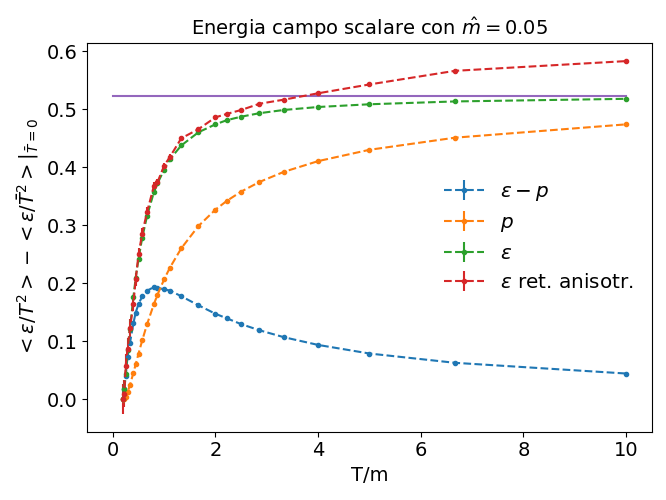
\includegraphics[width=\linewidth]{../figure/trace_anomaly.png}
\caption{Anomalia di traccia, pressione ed energia del campo al variare
della temperatura. In rosso l'energia calcolata con il metodo diretto
(reticolo anisotropo).}
\label{campo_scalare_trace_anomaly}
\end{figure}


\section{Teoria di pura gauge}
Abbiamo infine simulato la teoria di pura gauge U(1), interessati dalle proprietà
topologiche del modello.
Definendo come quantità elementari i trasporti paralleli fra punti del reticolo: $U_{\mu}(n)$ è
il trasporto parallelo del campo di gauge fra il punto $n$ e il punto
$n + \hat{\mu}$, dove il punto $n + \hat{\mu}$ ha le stesse coordinate del punto
$n$, ma con la coordinata in direzione $\hat{\mu}$ aumentata di uno.

Definiamo la placquette $\Pi_{\mu\nu}$ come il trasporto parallelo del campo di
gauge intorno ad un percorso chiuso in direzione prima $\mu$ poi $\nu$:
\begin{equation}
\Pi_{\mu\nu} = U_{\mu}(n) U_{\nu}(n+\hat{\mu}) U^*_{\mu}(n+\hat{\nu}) U^*_{\nu}(n)
\end{equation}
e usiamo come azione
\begin{equation}
S_E^L = \beta \sum_n \left( 1-\Re \Pi_{12}(n) \right)
\end{equation}
dove per confronto con la teoria al continuo ho $\beta = 1 / (g^2 a^2)$.

Allora possiamo usare il formalismo del path integral per simulare questa teoria
di campo.
In questa teoria la costante di accoppiamento $g$ non rinormalizza, per cui
il limite al continuo a volume costante si ottiene per $\beta \rightarrow \infty$
con $N_s N_t / \beta = cost$.


\paragraph{Suscettività a temperatura nulla}
Lavorando a temperatura nulla terremo sempre $N_s=N_t$.
Inoltre è stato scelto $T/g = 1 / 4$, temperatura abbastanza vicina allo zero,
per consentendo lo svolgimento dell'esperimento in tempi non proibitivi.

La quantità che andiamo a calcolare con le simulazione è la carica topologica.
\begin{equation}
Q = \frac{1}{2 \pi} \sum_n \arg(\Pi_{12}(n))
\end{equation}

Definendo quindi la suscettibilità topologica
\begin{equation}
\chi = \frac{\left< Q^2 \right> - \left< Q \right>^2}{V}
\end{equation}
A temperatura nulla la risoluzione analitica del modello prevede
\begin{equation}
\chi = \frac{g^2}{4 \pi}
\end{equation}

\paragraph{Algoritmo di simulazione e scelta dei parametri}
Come algoritmo di simulazione abbiamo questa volta eseguito un metropolis
seguito da N overrelaxations, e abbiamo concluso che il numero ottimale di
overrelaxations per diminuire la correlazione fra la misure fosse $N=1$.
In particolare fissato $T/g = 1 / 4$, $N_t=N_s=8$, abbiamo fatto 120 K updates
di metropolis.

\begin{center}
\begin{tabular}{ c | c | c | c }
\label{benchmark_U1gauge_field}
$N^{\circ}$ overrelaxation & tempo impiegato (s) &
$\tau_{int}$ per $N_t = N_s = 8$ \\
\hline
0 & 40 & 333 & 4381 \\
1 & 54 & 452 & 4500 \\
2 & 86 & 395 & 6435 \\
\end{tabular}
\end{center}

Nell'algoritmo metropolis abbiamo eseguito una spazzata di tutto il reticolo
nella direzione temporale a fissata variabile spaziale e quindi sulle variabili
spaziali, aggiornando prima il trasporto parallelo del sito n-esimo
in direzione spaziale e poi in quella temporale.
Abbiamo comunque verificato che ciò fosse equivalente a estrarre a caso
un sito del reticolo.

Innanzitutto vediamo che delta abbiamo scelto per il metropolis.
Sebbene per mantenere costante l'accettanza del metropolis al variare di $N_t$,
bisogni $\Delta \propto 1 / N_t^2$, questa non è sperimentalmente la scelta
migliore per ridurre l'autocorrelazione.

Abbiamo scelto $\delta = \pi$ anche se questo porta ad una bassa accettanza per
$N_t$ grandi, per minimizzare il tempo di autocorrelazione (e quindi l'errore)
della catena di Markov. Comunque per i nostri valori dei parametri,
l'accettanza è scesa al più a $\sim 3 \%$.

\paragraph{Risultati}
Per vari $N_t$ abbiamo runnato la simulatione e riportato la suscettibilità
in figura \ref{U1gaugefield_suscettivity}, la linea continua è il valore teorico
atteso della suscettibilità a $T=0$.
Abbiamo usato le tecniche di stima dell'errore spiegata largamente nel modulo 1,
in particolare l'errore sulla suscettibilità è stato calcolato con bootstrap
migliorato, a riguardo si veda figura \ref{U1gaugefield_bootstrap_migliorato}.

\begin{figure}
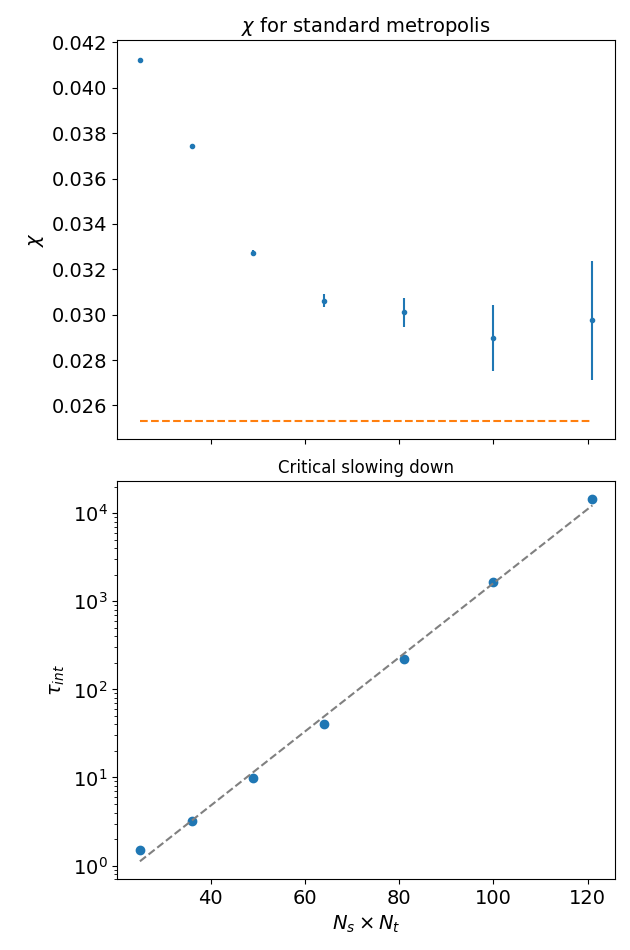
\includegraphics[width=\linewidth]{../figure/suscettivity.png}
\caption{Suscettività del campo al variare di $N_t \times N_s$,
con $N_t \times N_s / \beta = cost$, facendo il limite al continuo.
La linea continua mostra il valore teorico atteso (T=0).}
\label{U1gaugefield_suscettivity}
\end{figure}

\begin{figure}
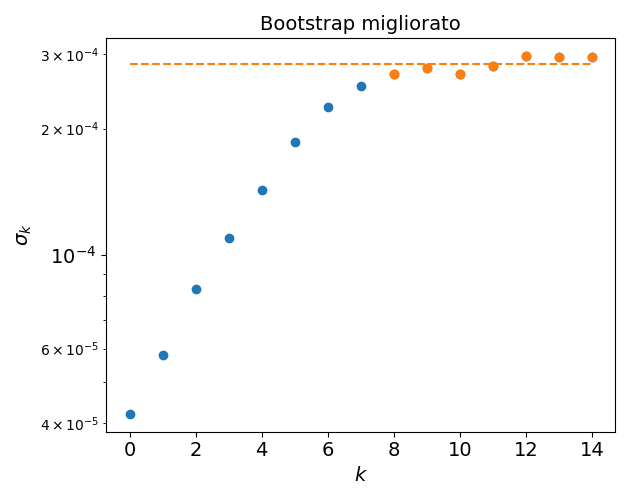
\includegraphics[width=\linewidth]{../figure/bootstrap_migliorato8.png}
\caption{Errore stima dal bootstrap al variare dei blocchi su cui medio.
Ottenuto per $N_t=8$, con 1.1 M di misure prese.
\'E stato fatto un fit nella regione dove l'errore non dipende più sensibilmente
dalla dimensione dei blocchi di misure su cui medio, i cui punti sono in arancione.}
\label{U1gaugefield_bootstrap_migliorato}
\end{figure}


Notiamo inoltre, cosa che si osserva dagli errori riportati in figura
\label{U1gaugefield_suscettivity}, che calcolando la sucettibilità topologica,
analogamente a quanto successo nel modulo 3, nel limite al continuo soffriamo
di critical slowing down ($\tau_{int} \propto e^{N_t \times N_S}$).
In figura \ref{U1gaugefield_autocorrelazione} riportiamo il tempo di autocorrelazione
della carica topologia Q al variare di $N_t \times N_S$.

\begin{figure}
\includegraphics[width=\linewidth]{../figure/autocorrelazione.png}
\caption{Tempo di autocorrelazione di Q del campo al variare di $N_t \times N_s$,
con $N_t \times N_s / \beta = cost$, facendo il limite al continuo (T=0).}
\label{U1gaugefield_autocorrelazione}
\end{figure}

\paragraph{Slab-method per rallentare la divergenza del tempo di autocorrelazione}
Per ovviare al critical slowing down si è pensato di applicare un algoritmo
differente, come quanto mostrato nel modulo 3.
Si è in particolare scelto di cercare di ricostruire la suscettività, nelle run
con Q identicamente nullo, a partire dalle misure di Q in un sottovolume, dove
Q non è più costretto ad essere un intero.

L'idea del metodo è la seguente:
conoscendo la probabilità di misurare carica topologica $Q$, sul volume $V$: $p(Q)_V$
la probabilità che sul sottovolume $xV$, $x \in (0,1)$ la carica topologica sia
$\tilde{Q}$ (non necessariamente intero) è
\begin{equation}
p(\tilde{Q})_{xV} \times p(Q - \tilde{Q})_{(1-x)V}
\end{equation}

Assumendo che $p(Q)_V \propto e^{-Q^2 / (2 \chi V)}$, e posto $Q=0$ sul volume totale,
\begin{equation}
\chi_s = \frac{\left< Q^2 \right>_{xV}}{V} = \chi x (1-x)
\end{equation}

Possiamo cioè ricostruire il vero valore di $\chi$ sul volume
fittando una parabola sulle misure di $\chi_s$ su una frazione del volume

Per essere sicuri di avere $Q$ identicamente nullo, si è scelta di partire 'a freddo',
cioé tutti i trasporti paralleli avevano inizialmente lo stesso valore.
Poi si è termalizzato, cioé si è fatto evolvere il sistema senza prendere misure,
abbastanza a lungo che perdesse memoria delle condizioni iniziali.
Ed sono stati scelti valori di $N_t$ sufficentemente grandi per cui non ci
aspettavamo cambiamenti di Q, questo è stato verificato anche a posteriori.

Per avere una migliore sensibilità sulla divisione si è rinunciato a tenere
$N_s = N_t$, e si è fissato $N_s$ pari ad un multiplo di 10,
in particolare $N_s = 20$, per dividere il volume in blocchi da 10.

Un esempio di tale fit ottenuto per $N_t = 0$ si vede in figura
\ref{suscettivity_fit}.

\begin{figure}
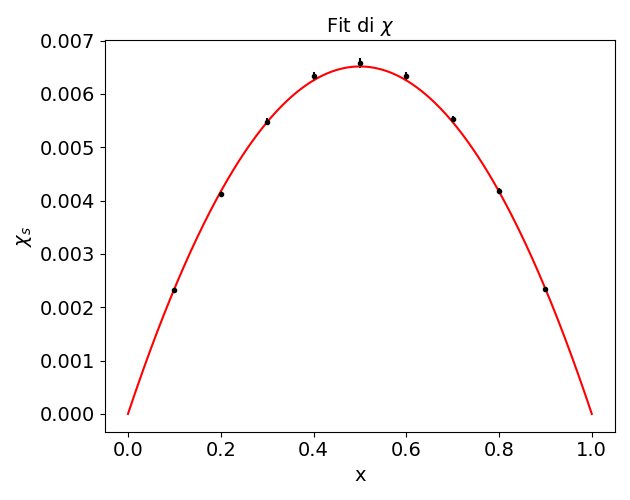
\includegraphics[width=\linewidth]{../figure/suscettivity_fit17.png}
\caption{Fit della suscettività dalle misure sui sotto volumi
secondo la formula $x(1-x) \chi$}
\label{suscettivity_fit}
\end{figure}

Vediamo che il tempo di autocorrelazione di Q è molto migliorato,
essendo simmetrico in $x$ e $1-x$, mostriamo il tempo di autocorrelazione
per $x=0.1$ e $x=0.2$, in figura \ref{autocorrelation_time_slab}.

\begin{figure}
\includegraphics[width=\linewidth]{../figure/autocorrelation_time_slab.png}
\caption{Tempo di autocorrelazione di Q, calcolato in $x=0.1$ e $x=0.3$ frazione
del volume totale $xV$}
\label{autocorrelation_time_slab}
\end{figure}

Vediamo infine la suscettività al variare di $N_t$ in figura \ref{suscettivity_slab}
\begin{figure}
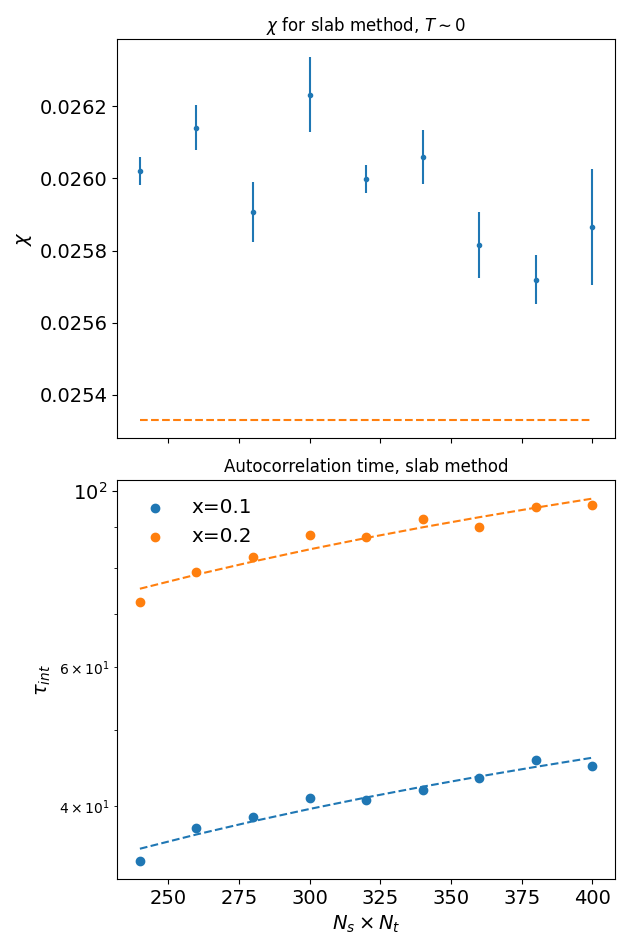
\includegraphics[width=\linewidth]{../figure/suscettivity_slab.png}
\caption{Suscettività al variare di $N_t$, calcolata usando lo slab method.
La linea continua rappresenta la previsione teoria a $T=0$.}
\label{suscettivity_slab}
\end{figure}

\end{document}
